
\documentclass[12pt]{amsart}
\usepackage{amssymb,amsmath}
\usepackage{graphicx}
\usepackage{geometry} % see geometry.pdf on how to lay out the page. There's lots.
\geometry{a4paper} % or letter or a5paper or ... etc
% \geometry{landscape} % rotated page geometry

\newcommand{\bigzero}{\mbox{\normalfont\Large\bfseries 0}}
\newcommand{\rvline}{\hspace*{-\arraycolsep}\vline\hspace*{-\arraycolsep}}


% See the ``Article customise'' template for come common customisations

\title{Visualizing Grover's Search Algorithm}
\author{James Weaver \& Paul Kassebaum}
\date{} % delete this line to display the current date

%%% BEGIN DOCUMENT
\begin{document}

\maketitle

\section{Oracle operators}

If we want an operator $U_x$ with the following behavior

\begin{equation}
	\begin{split}
		U_x |x\rangle & = - |x\rangle \\
		U_x |x_\perp\rangle & = |x_\perp\rangle 
	\end{split}
\end{equation}

where all $|x_\perp\rangle$ are orthogonal to $|x\rangle$, then the operator takes the form

\begin{equation}
	U_x = I - 2 |x\rangle\langle x|
\end{equation}

Let's demonstrate this with a couple of examples.

\begin{equation}
	\begin{split}
		U_x |x\rangle & = (I - 2 |x\rangle\langle x| ) |x\rangle \\
		& = |x\rangle - 2 |x\rangle\langle x | x\rangle \\
		& = |x\rangle - 2 |x\rangle \\
		& = - |x\rangle
	\end{split}
\end{equation}

because $\langle x | x\rangle = 1$.

\begin{equation}
	\begin{split}
		U_x |x_\perp\rangle & = (I - 2 |x\rangle\langle x| ) |x_\perp\rangle \\
		& = |x_\perp\rangle - 2 |x\rangle\langle x | x_\perp\rangle \\
		& = |x_\perp\rangle - 2 \langle x | x_\perp\rangle  |x_\perp\rangle \\
		& = |x_\perp\rangle
	\end{split}
\end{equation}

because $\langle x | x_\perp\rangle = 0$.

Now let's look at the result of acting on an arbitrary state $|\alpha\rangle$, that is not completely orthogonal to $|x\rangle$.

\begin{equation}
	\begin{split}
		U_x |\alpha\rangle & = (I - 2 |x\rangle\langle x| ) |\alpha\rangle \\
		& = |\alpha\rangle - 2 |x\rangle\langle x | \alpha\rangle \\
		& = (1 - 2 \langle x | \alpha\rangle)  |\alpha\rangle \\
	\end{split}
\end{equation}

In words, the result is the original state vector minus twice the overlap or projection of $|\alpha\rangle$ on $|x\rangle$. We can draw this out geometrically.
\begin{figure}[h]
   \centering
   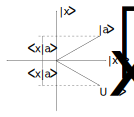
\includegraphics[width=0.5\textwidth]{./img/fig-00} % requires the graphicx package
   \caption{Geometric demonstration that the operator $U_x$ has the effect of reflecting $|\alpha\rangle$ across $|x_\perp\rangle$, the vector orthogonal to $|x\rangle$.}
   \label{fig:example}
\end{figure}




\section{Symmetries of a single qubit system}
A single qubit's state $|s\rangle$ 

\begin{equation}
	|s\rangle = (a+ib)|0\rangle + (c + id)|1\rangle
\end{equation}

written in terms of the 4 real numbers $a,b,c,d$ can be fully described by 3 real numbers, since the state must be normalized,

\begin{equation}
	\langle s | s\rangle = a^2 + b^2 + c^2 + d^2 = 1,
\end{equation}

which makes one of the real numbers dependent on the other three.

A single qubit's rotational symmetries can be described by the matrices

\begin{equation}
	\begin{pmatrix}
		a + i b & -(c - id) \\
		c + id & -(a + i b)
	\end{pmatrix}
\end{equation}

where $a,b,c,d$ are real numbers. The normalization condition on the state of the qubit requires that the determinant of this matrix be 1. 

Another way to describe a single qubit's rotational symmetries is by the quaternion:

\begin{equation}
	a +bi + cj + dk
\end{equation}

where the real numbers $a,b,c,d$ of the matrix and quaternion are equal respectively. The determinant of the matrix is the norm of the corresponding quaternion. Since the matrix has determinant 1 as a consequence of the normalization condition of the qubit's state, the corresponding quaternion has norm 1.


\section{Symmetries of a two qubit system}

A system of two qubits can be described by $2\times3 = 6$ real numbers. The system transforms as the tensor product of two independent matrices that each describe a single qubit, as explained above.

\begin{equation}
	\begin{pmatrix}
  \begin{matrix}
  i a & -\bar{z} \\
  z & - i a
  \end{matrix}
  & \rvline & \bigzero \\
\hline
  \bigzero & \rvline &
  \begin{matrix}
  i b & -\bar{w} \\
  w & -i b
  \end{matrix}
\end{pmatrix}
\end{equation}

where $a,b$ are real numbers and $z,w$ are complex numbers. The numbers $a,z,b,w$ are made up of 6 independent real numbers. Each of the two block matrices can be related to independent quaternions.

The dynamics of a two qubit system can be thought of geometrically in 4D euclidean space where each of the two quaternions is acted upon independently by operators associated with each spin respectively.




\end{document}